I focus on a string of episodes where Jane, a promising trench assistant working at an archaeological project, learned to identify, differentiate, and document parts of a stratigraphic sequence.
I illustrate how the constitution of the archaeological record, and the internalization of archaeological knowledge, occurred as part of project frameworks and collaborative relations that were structured by projects' divisions of labour.

\subsection*{Learning to see like an archaeologist}
As illustrated in \autoref{fig:context-change}, Jane explained to me how she identified and differentiated a new context that she was beginning to expose in her trench, using a series of gestures paired with speech to help convey what she meant to say.\textsuperscript{\ref{A1}}
Jane kicked the boulders as she referred to them, literally pointed out relations to previous experiences that she deemed relevant, and described certain aspects of the soil by miming the ways that she would interact with them.
She referred to common nomenclature outlined in the project's excavation manual, and drew from her experiences working in other trenches that others may have shared.
More generally, she described the context change only in terms of her interactions with it, and as framed by her particular role in the project.

\begin{sidewaysfigure}
\centering
\setlength{\fboxsep}{1pt}
\setlength{\fboxrule}{1pt}
\fbox{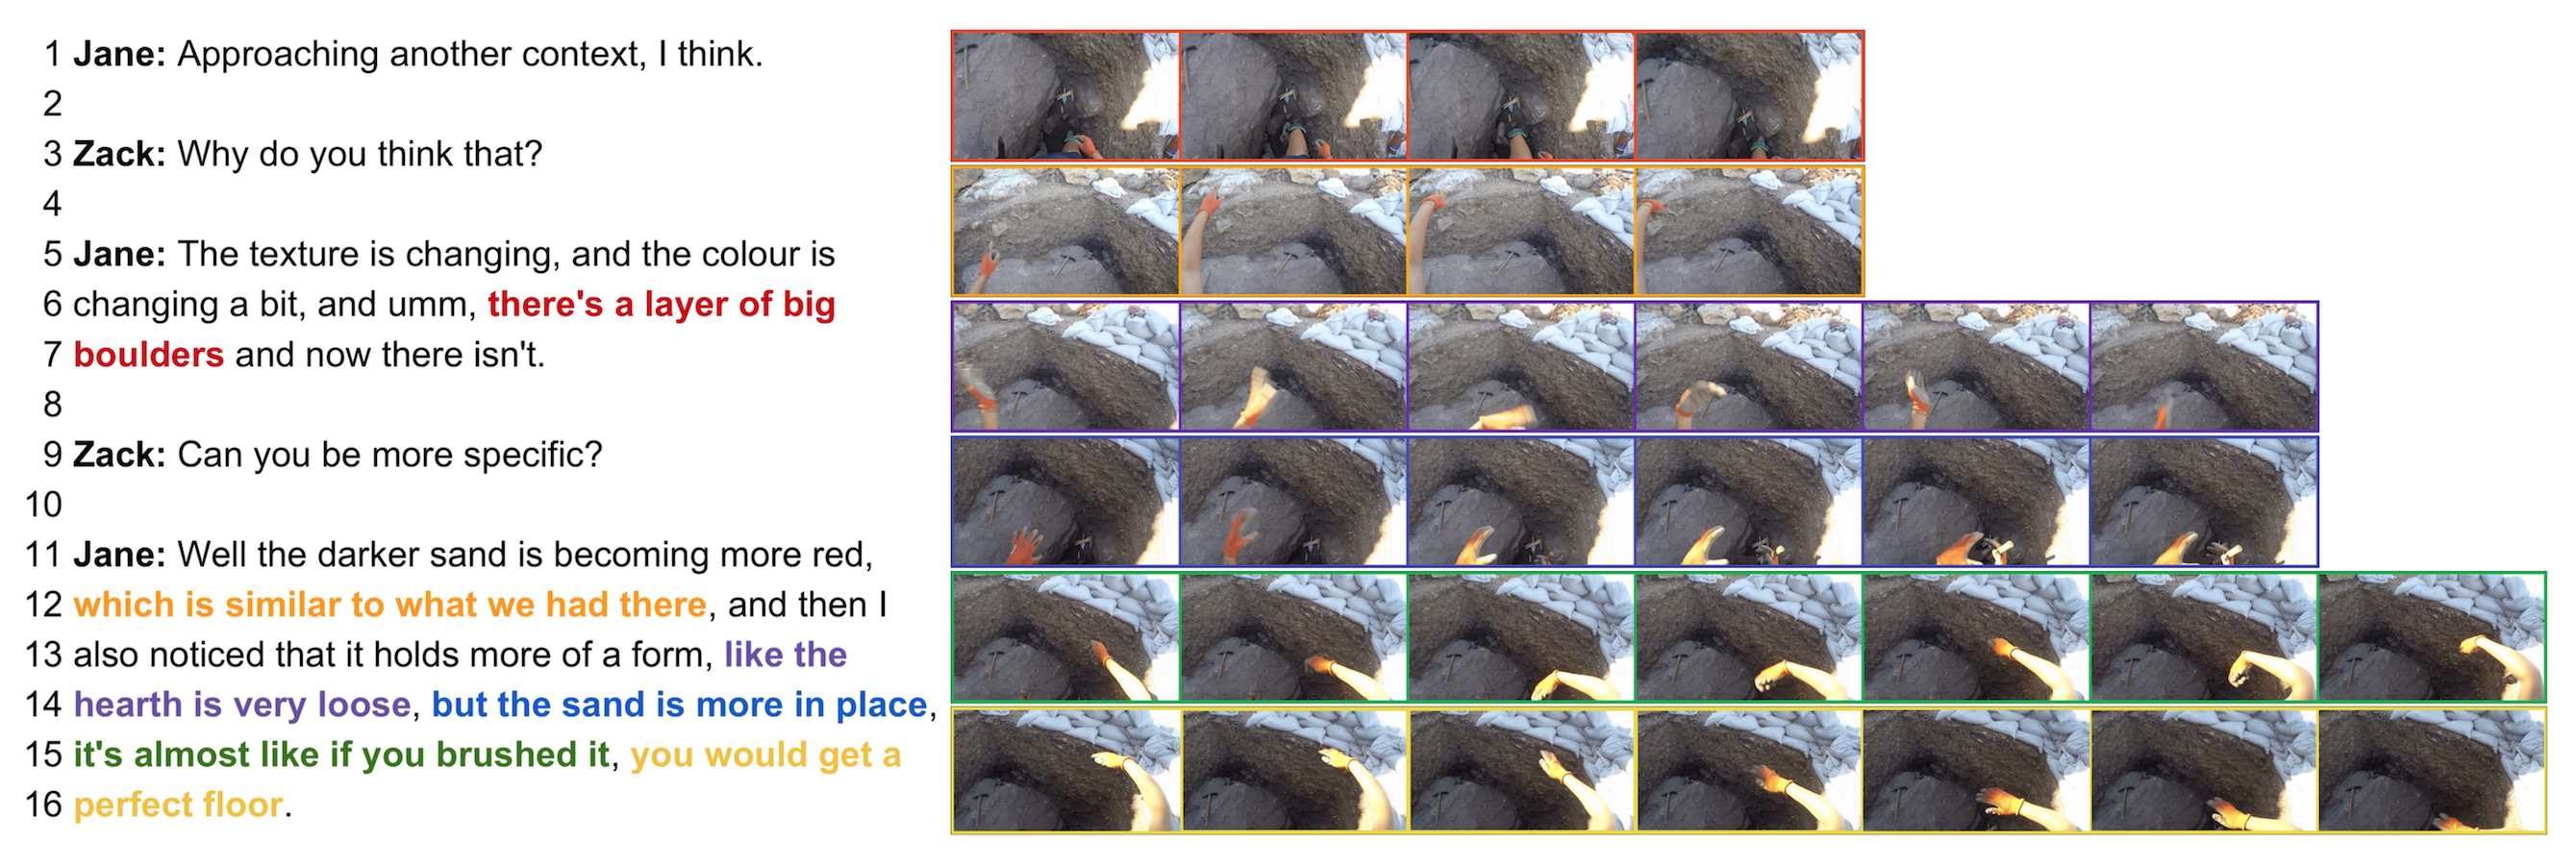
\includegraphics[width=0.99\textwidth]{context-change.png}}
\caption[Explanation of a potential context change using gestures and speech.]{Explanation of a potential context change using gestures and speech.}
\label{fig:context-change}
\end{sidewaysfigure}

Afterward, and as illustrated in \autoref{fig:context-change-discussion}, Jane consulted with Basil, who supervised work in this trench, and who is also the project director, regarding her interpretation of the soil in it.\textsuperscript{\ref{A2}}
Jane explained what she saw, in terms of her encounters with the entities she identified, while punctuating her observations with physical gestures that underscored certainty that the entities she was observing actually exist.
Basil came to take a closer look and translated Jane's situated experiences into more nominal and normalized terms, that distance the observer from the observed entities.
Basil then identified a series of actions that Jane must implement, and summarized the situation by joining what was observed with what was to be done about it, in effect rendering a conclusive and well-reasoned decision.
All the while, Jane confirmed her understanding of Basil's corrections and of his specific instructions.

\begin{sidewaysfigure}
\centering
\setlength{\fboxsep}{1pt}
\setlength{\fboxrule}{1pt}
\fbox{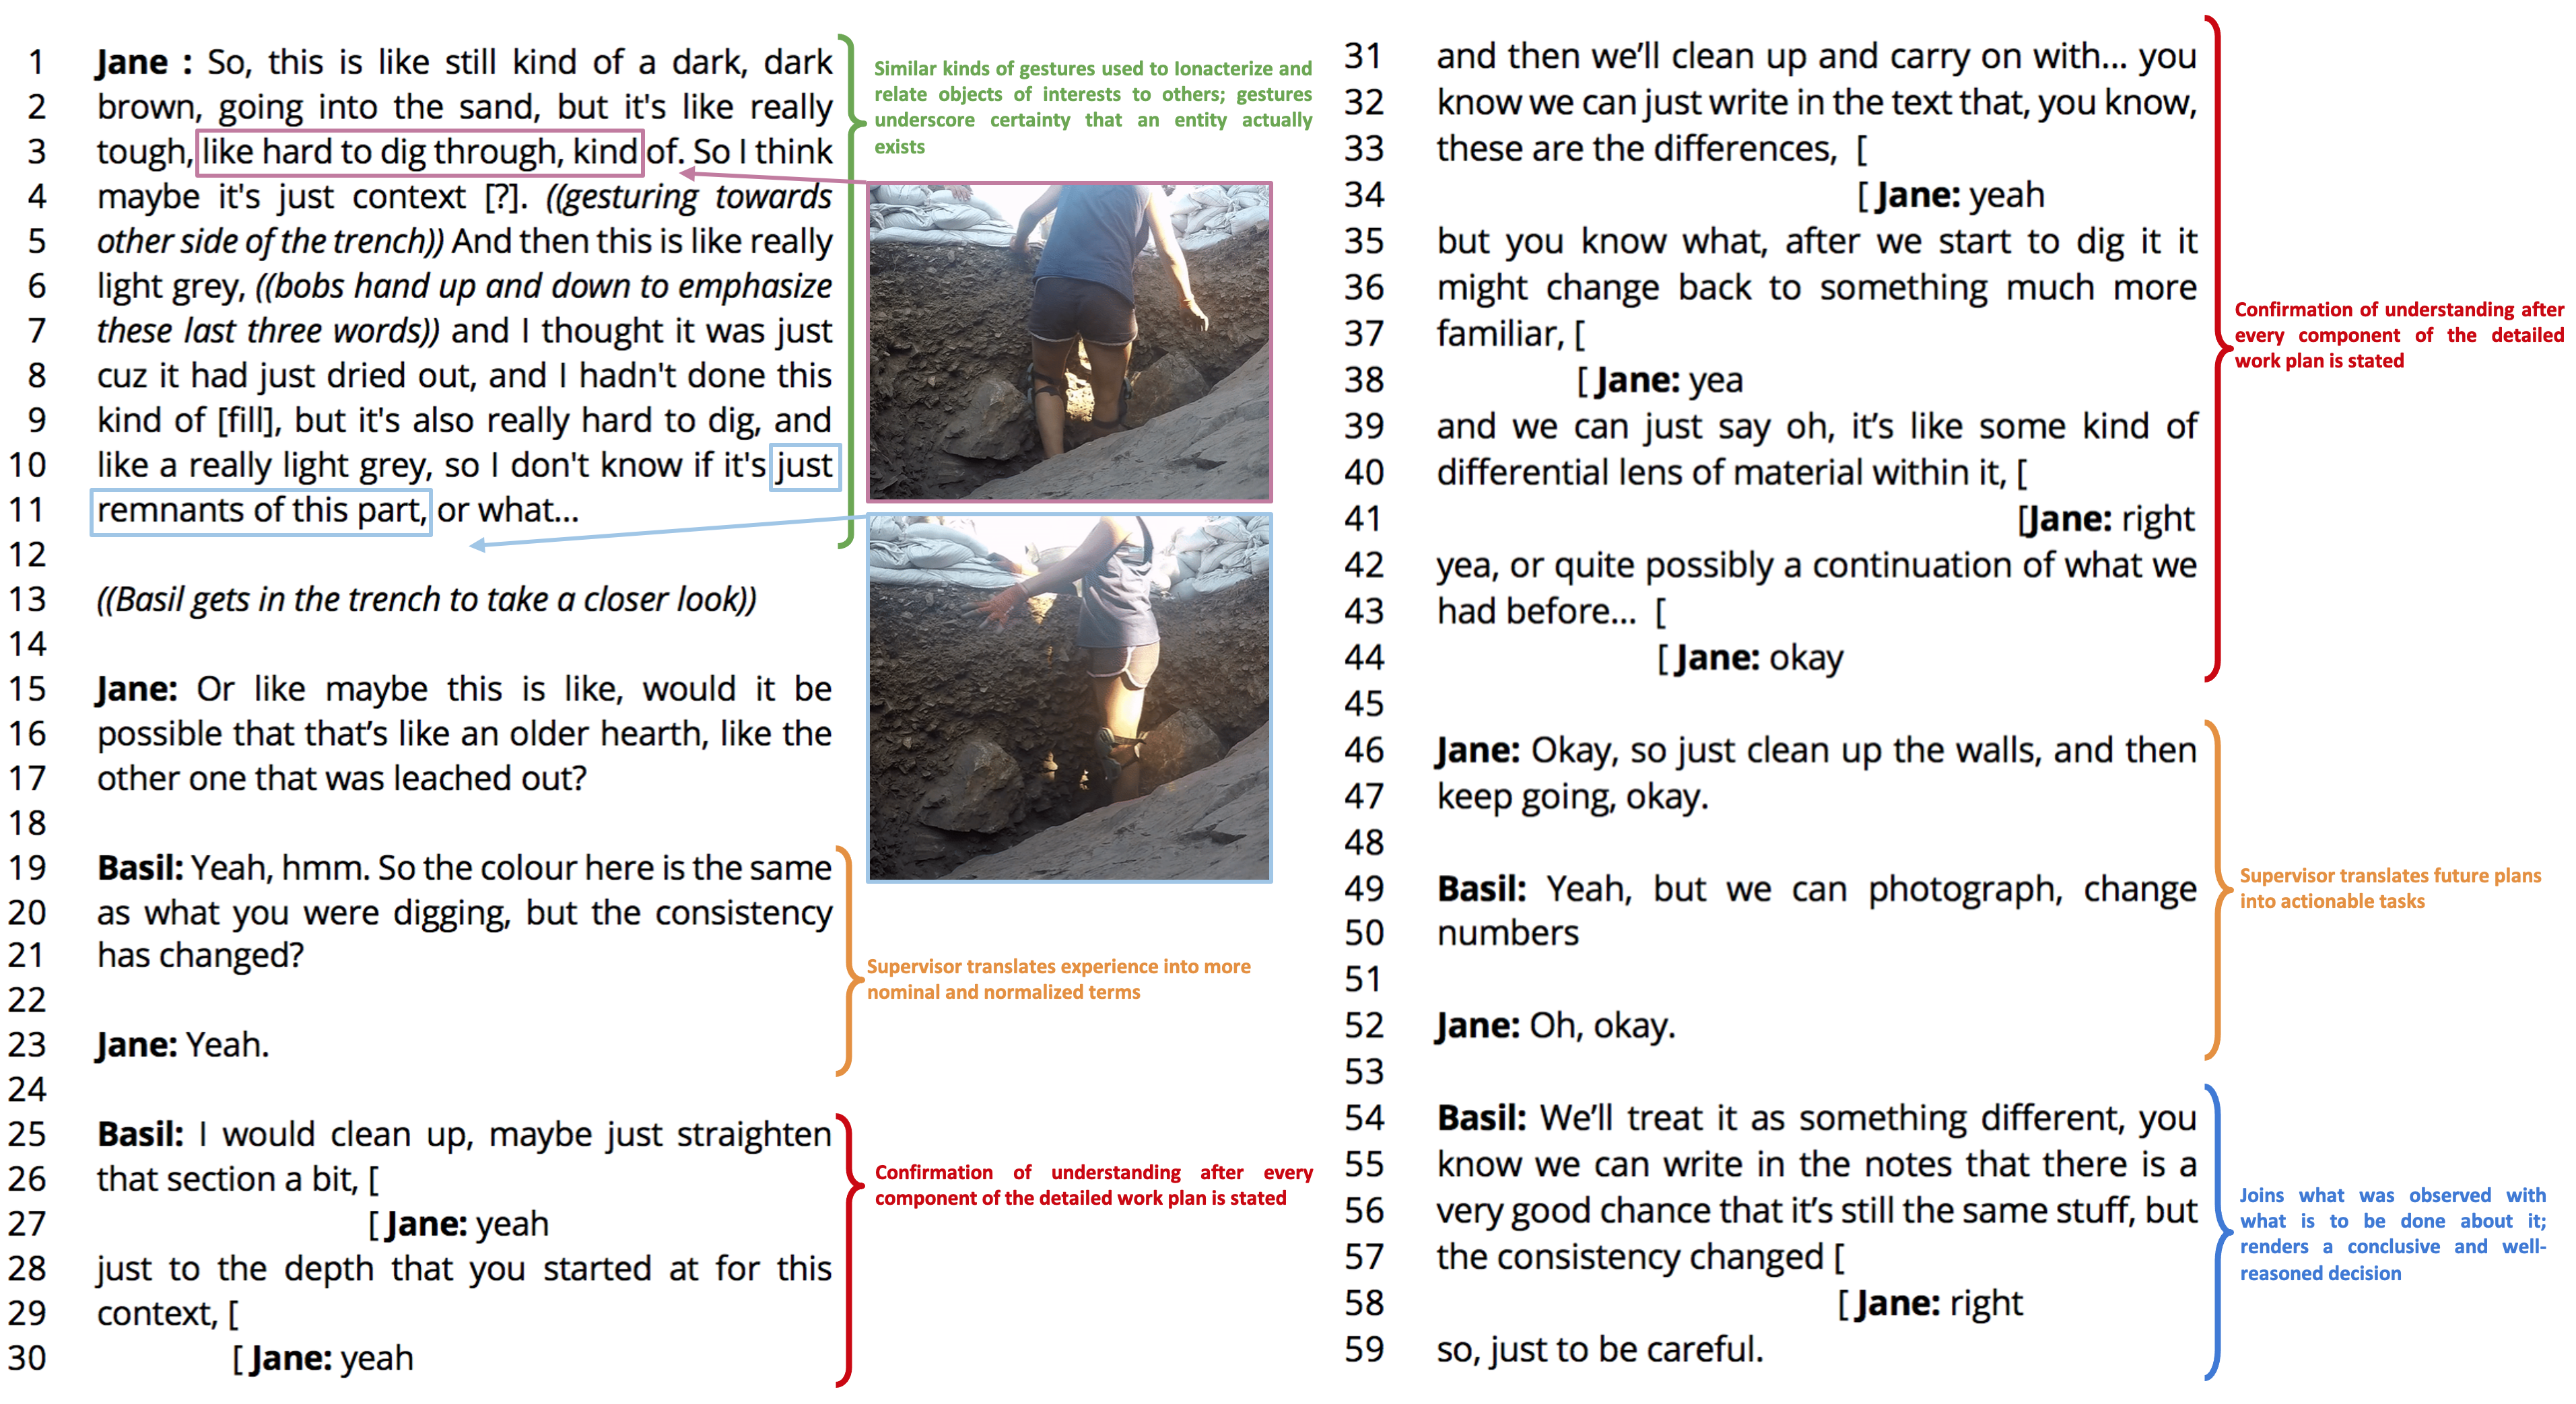
\includegraphics[width=0.99\textwidth]{context-change-discussion.png}}
\caption[Discussion of a potential context change using gestures and speech.]{Discussion of a potential context change using gestures and speech.}
\label{fig:context-change-discussion}
\end{sidewaysfigure}

When Jane explained her interpretation of the soil to her supervisor, he then responded with tentative agreement, paired with his own gestures and intonations that subtly communicated his agreement or disagreement.
The conversation between Jane and Basil therefore served as a means of calibrating their experiences, using an independent framework as a common reference point.
In effect, Basil attempted to align Jane's emerging perspective with professional nomenclature used to describe the sediment's character.

As Jane stated in a subsequent interview (\autoref{fig:training-eye}), she initially found it difficult to ``train her eye to see what they're seeing'', and ``they'' seems to refer to more senior and specialized archaeologists, including her supervisor the director, and Alfred, one of the field directors.\textsuperscript{\ref{A3}}
By talking through their observations in an explicit manner and in the presence of the entities of mutual concern, while also referencing concrete characteristics of the soil, Basil trained Jane to see things in a way that corresponds to a formal model of how to differentiate soil, and contexts as an natural extension of that ability.
This made him more confident in Jane's ability to recognize and report her experiences, upon which Basil depends; as he recalled in a separate interview, Basil came to trust Jane ``to either make her own decisions or be responsible enough to ask other people to help her make decisions for those moments when I'm not there.''\textsuperscript{\ref{A4}}
This was because Jane became capable of deciding for herself when and how to distinguish between sediments, having internalized a conceptual framework that affords professional legitimacy to her observational techniques.

\begin{figure}[H]
  \centering
  \setlength{\fboxsep}{1pt}
  \setlength{\fboxrule}{1pt}
  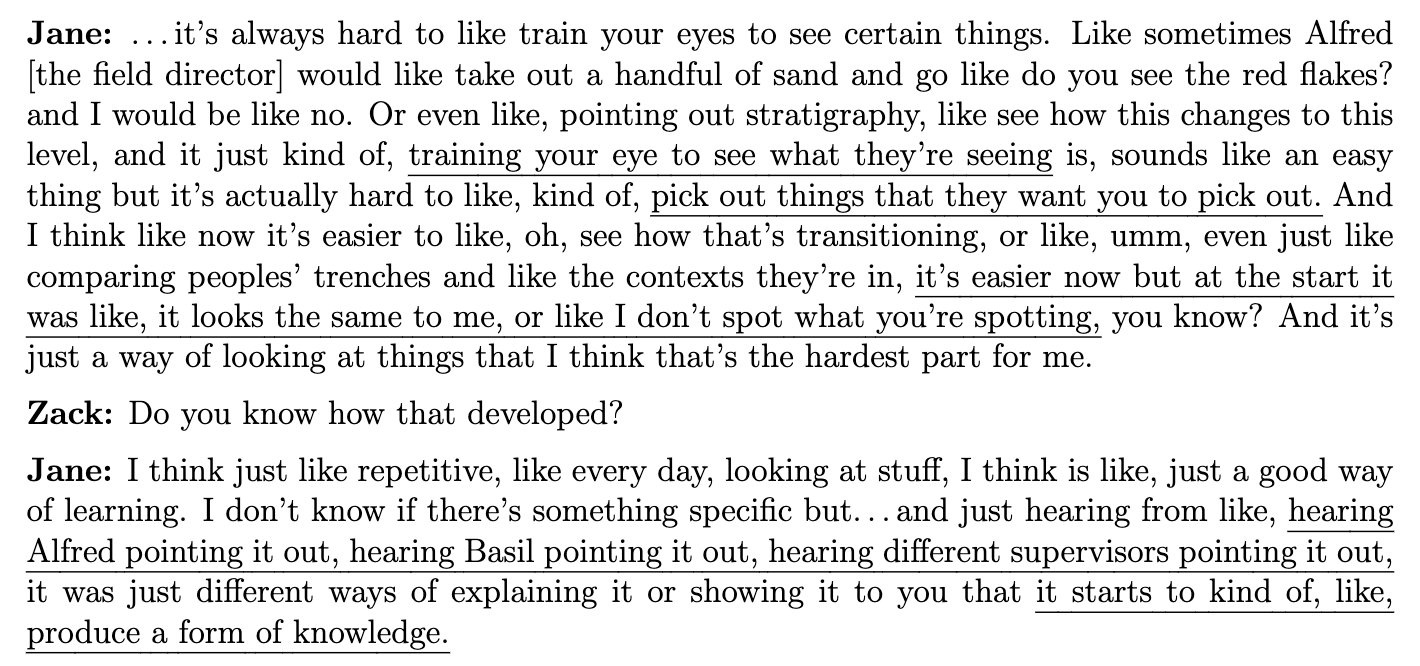
\includegraphics[width=0.99\textwidth]{training-eye.png}
  \caption{Jane describes how she learned to recognize differences in the soil.\textsuperscript{\ref{A3}}}
  \label{fig:training-eye}
\end{figure}

% \begin{quote}
%   \textbf{Jane:} \dots it's always hard to like train your eyes to see certain things. Like sometimes Alfred [the field director] would like take out a handful of sand and go like do you see the red flakes? and I would be like no. Or even like, pointing out stratigraphy, like see how this changes to this level, and it just kind of, \ul{training your eye to see what they're seeing} is, sounds like an easy thing but it's actually hard to like, kind of, \ul{pick out things that they want you to pick out.} And I think like now it's easier to like, oh, see how that's transitioning, or like, umm, even just like comparing peoples' trenches and like the contexts they're in, \ul{it's easier now but at the start it was like, it looks the same to me, or like I don't spot what you're spotting,} you know? And it's just a way of looking at things that I think that's the hardest part for me.\\[0.5em]
%   \textbf{Zack:} Do you know how that developed?\\[0.5em]
%   \textbf{Jane:} I think just like repetitive, like every day, looking at stuff, I think is like, just a good way of learning. I don't know if there's something specific but\dots and just hearing from like, \ul{hearing Alfred pointing it out, hearing Basil pointing it out, hearing different supervisors pointing it out,} it was just different ways of explaining it or showing it to you that \ul{it starts to kind of, like, produce a form of knowledge.} \textsuperscript{\ref{A3}}
% \end{quote}

\subsection*{Shedding the body}
I should note that Jane did not actually object to the reduction of her situated experience in favour of more generic forms of representing the stratigraphy.
In fact, this conformed with a pattern of behaviour -- which was enacted by all the fieldworkers I spoke with -- whereby they tried not to think too much while excavating, opting instead to operate in the moment, responding only to what was directly in front of them.\textsuperscript{\ref{A5}, \ref{A6}}
This conformed with the expectation that the things an excavator uncovers will gradually reveal themselves, and that she should passively follow what is occurring in the earth before her.

To help accomplish this, fieldworkers modified the environments in which they worked.
For instance, some fieldworkers focused better while listening to music or while blocking out social distractions.\textsuperscript{\ref{A7}, \ref{A8}}
Ben, who worked as an assistant in a separate trench, said that listening to music helped him avoid being too self-aware\textsuperscript{\ref{A7}} while Jane concurred by expressing that she listened to music to help her ``get lost in digging.''\textsuperscript{\ref{A8}}
Even when music was not used, or when it is forbidden on site, there remains a warrant for fieldworkers to remain focused as they work.\textsuperscript{\ref{A9}}
For instance, Basil recalled what he characterized as ``old fashioned'' archaeological fieldwork practices, which dictate that ``the only sound you should hear is trowel on stone.''\textsuperscript{\ref{A8}}

Having all the necessary tools at hand was another way to facilitate uninterrupted focus during fieldwork.\textsuperscript{\ref{A10}}
This helped eliminate peripheral sensory distractions when getting up or reaching for tools placed further away.
In effect, fieldworkers were made to become disembodied sensing devices attuned to one thing and one thing only: the soil immediately in front of them.
This notion was further underscored by my unrecorded but common observations of supervisors having to force assistants to take breaks, drink water, apply sunscreen, and remind them that they have bodies worth cherishing and protecting.

In some cases, fieldworkers found certain kinds of information useful as they excavated.
For instance, knowing about similar stratigraphy in nearby trenches enabled excavators to work at a quicker pace, since it this provided a general understanding of the order and depth of the stratigraphy under them.\textsuperscript{\ref{A11}, \ref{A12}}
Moreover, when finds specialists reported back to fieldworkers about the contents of their ongoing trenches, their preliminary findings sometimes influenced the care with which they excavated and recorded the trench.\textsuperscript{\ref{A13}, \ref{A14}}
While Theo (a trench supervisor who eventually became a field director) indicated that knowing about the properties of lithic artefacts that lithics specialists deemed important helped him undertake his work in a manner that better suited the project's overall aims, he presented this notion in very broad terms, and refrained from indicating specific practical impacts when prompted. \textsuperscript{\ref{A13}}
Moreover, Ben dismissed the input provided by palaeobotanical experts as useless to him because he was unable to ``see'' the archaeobotanical traces as he worked.\textsuperscript{\ref{A15}}
This may merely reflect practical concerns, specifically regarding the microscopic nature of properties that render archaeobotanical remains significant, but it would not be absurd to find ways to help fieldworkers make sense of such insights in the field.
For instance, fieldworkers may carry a magnifying loupe and reference guide, and be trained to understand how to use them, similar to how Jane learned to characterize soil samples in the field.
However, this would require a more comprehensive partnership between specialists and fieldworkers, and broadening the extreme focus that fieldworkers have honed for themselves.

In general then, I observed aspects of fieldwork practice that both complement and contradict efforts to enhance reflexivity in fieldwork.
The professed desire not to overthink while excavating pushes back against impulses to provide more information to fieldworkers during the moment of excavation \parencites(cf.)()[]{berggren2012}[]{berggren2015}.
According to Theo and Ben, fieldworkers operate in a strictly separate role than those who interpret and write about finds, and this boundary feels natural to them.\textsuperscript{\ref{A16}, \ref{A17}, \ref{A18}}
Rather than ingest loads of additional information, which involves learning how to make sense of it all and find it meaningful in a practical sense,\textsuperscript{\ref{A19}} the fieldworkers I spoke with went in the opposite direction; they value their extremely focused experiences with the material, which presents them with a unique and proprietary way of knowing that dissipates as they are, as Edgeworth \parencite*[109]{edgeworth2003} put it, forced to ``[detach themselves] from the task-in-hand to consider the material field from a distance''.
This means of engagement feels more natural to them, as if unmuddied by reflexive thought, and the fieldworkers I spoke with perceived this as a strength.

At the same time, the fieldworkers I spoke with were very aware that all observation is subjective and that all records carry biases imposed by the practical circumstances of their creation; they were deeply involved in navigating these practical circumstances and in devising ways to control their environments to foster the \emph{illusion} of objectivity.
All of what I described was in service of a broader systemic framework, which is informed by a (flawed) conception of the nature of archaeological data and of what constitutes proper or legitimate archaeological reasoning \parencite[]{batist-alienation}.

% In what follows, I will describe how the act of producing a record brings things back to situated reality, as well as attempts to ignore that reality.

\subsection*{Leaving traces in the subsequent record}
Turning back to the specific example, Basil's prediction that the context would not change came to fruition.
However, the tentative decision to proceed as if a change in context was imminent left residual traces on recording sheets, in the database, and in the final trench report (see \autoref{fig:context-description-transcribed} and \autoref{fig:context-sketch}).

% \begin{quote}
%   \textbf{Why did you change contexts?}\\
%   We think we are still within the hearth(?) feature but in the western half of the trench (i.e. that part not covered by a boulder) the sediment has changed somewhat. In NW quadrant the soil is still dark but is now more compact. In SW it is more compact and more grey.\\[1em]
%   \textbf{Context description:}\\
%   SW corner of trench where a grey (ashy?) compact soil. 100\% soil for flotation. Fewer artefacts. After a couple of centimetres it turns back into the black soil (i.e. this is now another arbitrary stratum in the hearth feature).
% \end{quote}

\begin{figure}[H]
  \centering
  \setlength{\fboxsep}{1pt}
  \setlength{\fboxrule}{1pt}
  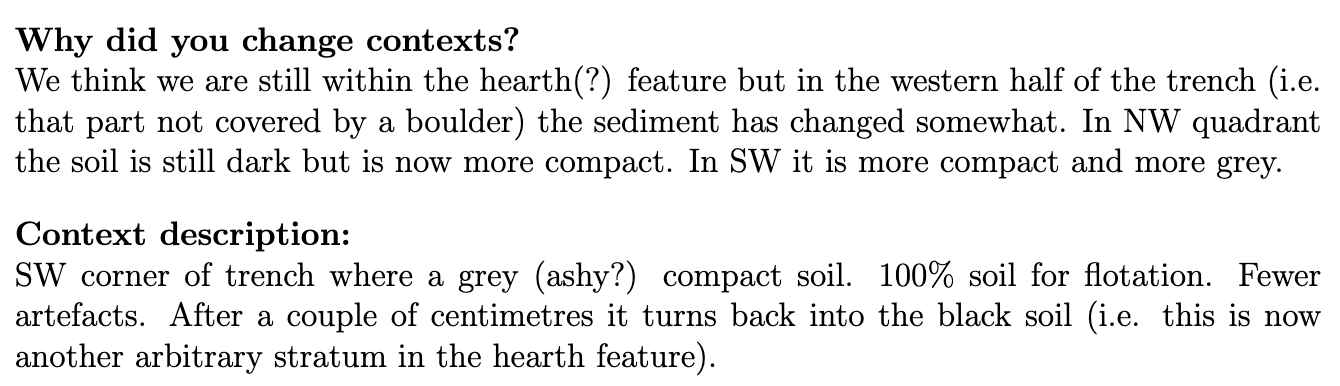
\includegraphics[width=0.99\textwidth]{context-description-transcribed.png}
  \caption{Transcribed section of a recording sheet describing the context addressed in the observed episode.}
  \label{fig:context-description-transcribed}
\end{figure}

% \begin{figure}[H]
% \centering
% \setlength{\fboxsep}{1pt}
% \setlength{\fboxrule}{1pt}
% \includegraphics[width=0.99\textwidth]{context-description.png}
% \caption[Section of a recording sheet describing a context.]{Section of a recording sheet describing a context.}
% \label{fig:context-description}
% \end{figure}

\begin{figure}[H]
\centering
\setlength{\fboxsep}{1pt}
\setlength{\fboxrule}{1pt}
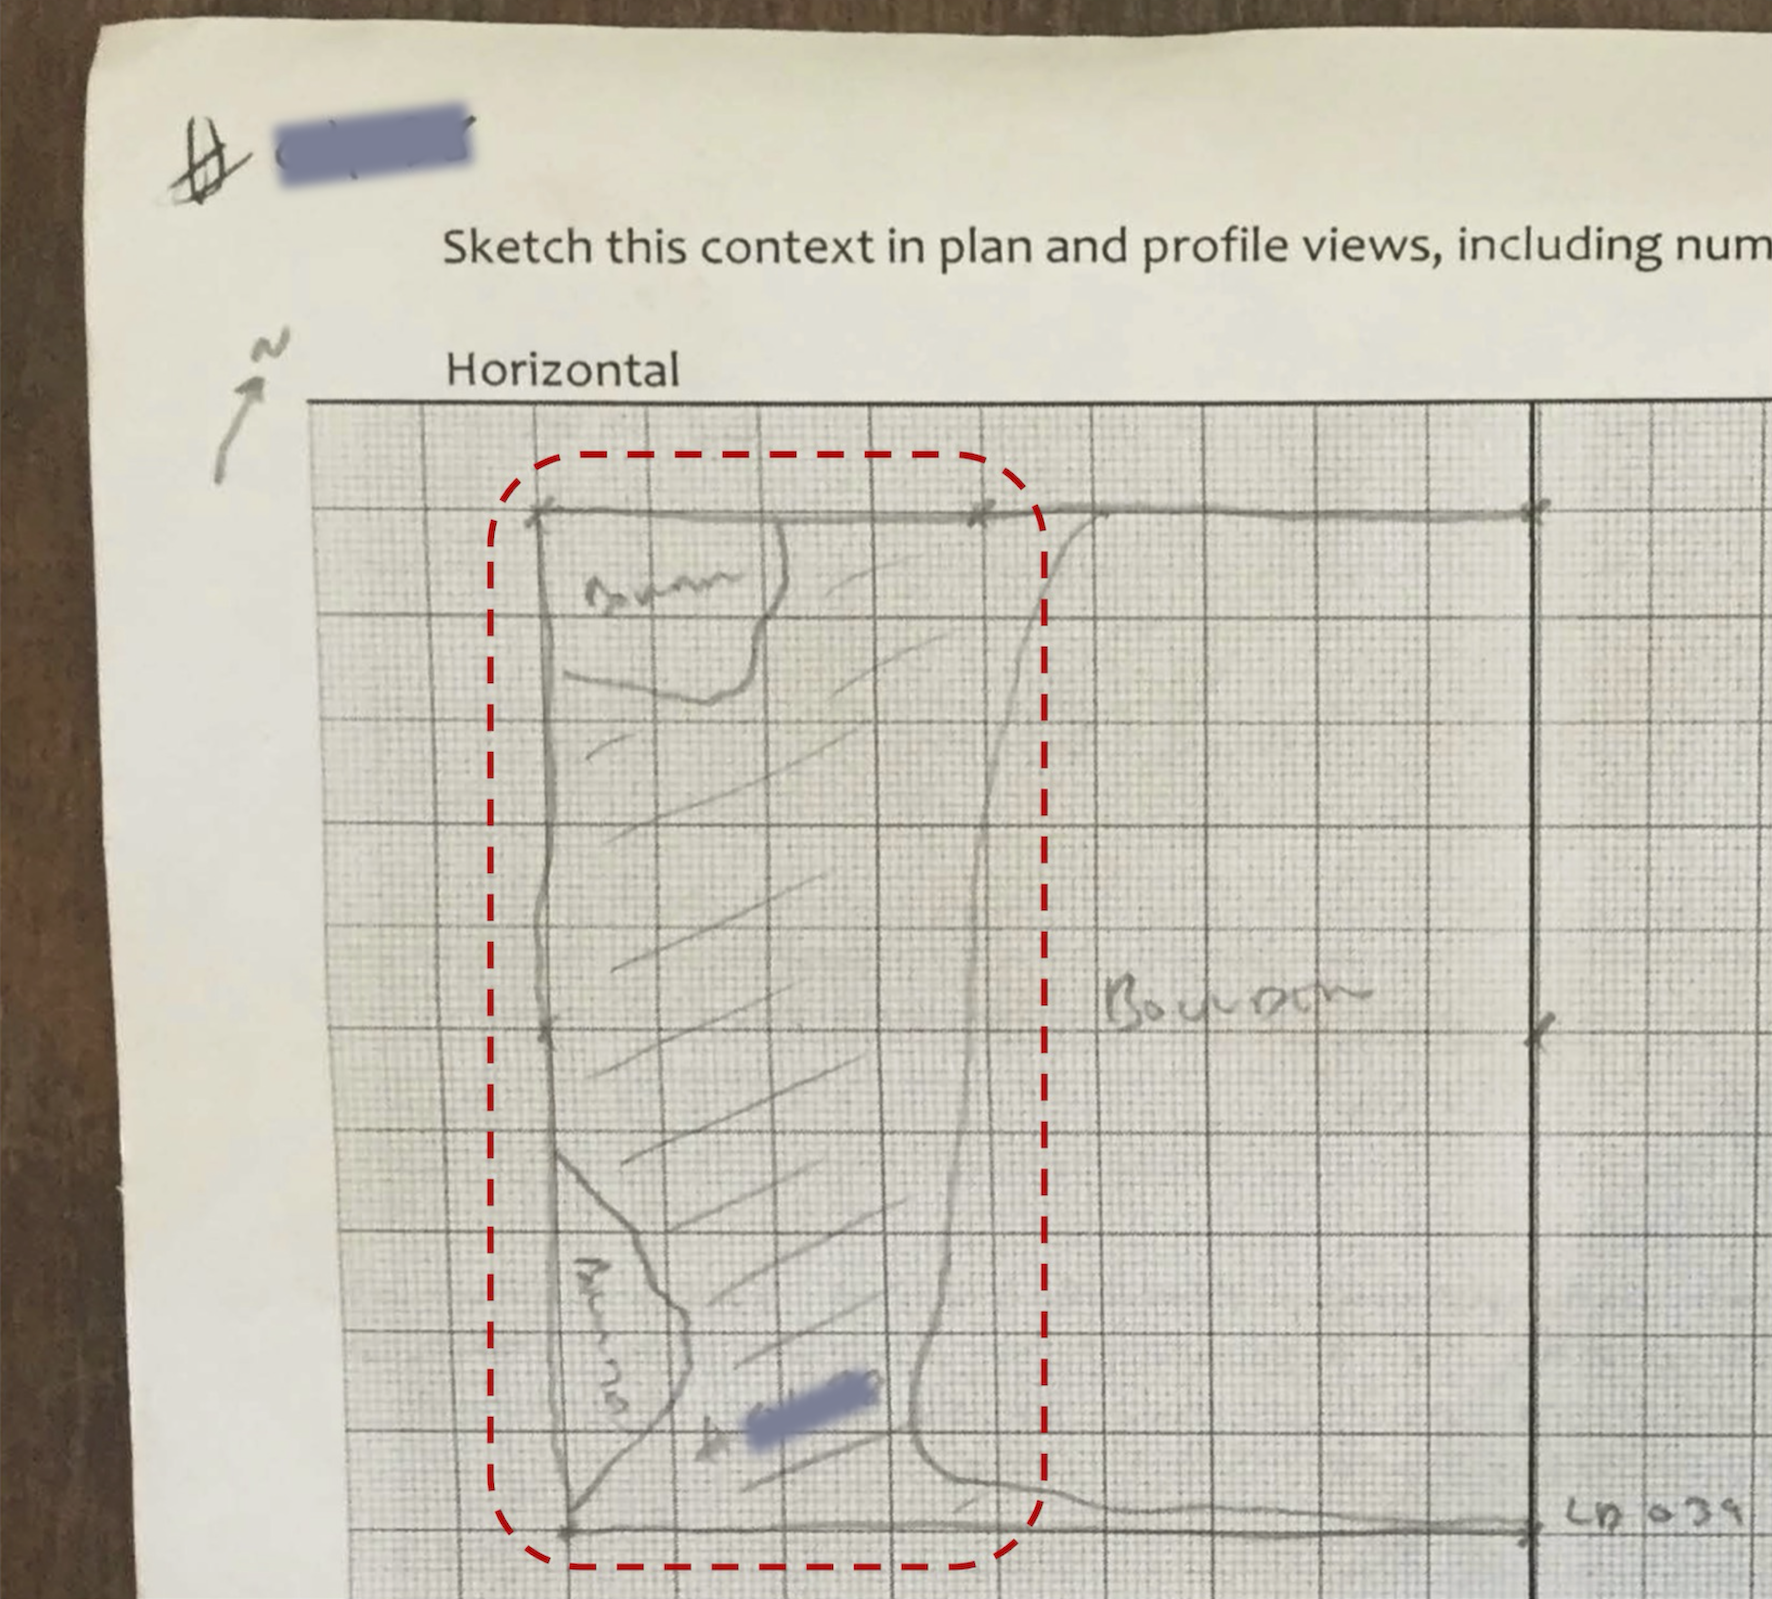
\includegraphics[width=0.99\textwidth]{context-sketch.png}
\caption{Sketch of the base of a trench, portraying the context addressed in the observed episode, boxed in red.}
\label{fig:context-sketch}
\end{figure}


% \begin{quote}
%   The sediment in this context had changed a bit but we assumed we were still within the hearth(s). It appeared more ashy so we described it as a new context. However, after a couple of centimetres it turned back to the darker soil so it was then decided that this was indeed a continuation of the hearth. It was then considered an arbitrary change of context. Overall, it was grey ashy soil with angular and fairly compact stones, it was medium/fine sand, poorly sorted, and 10YR 4/1. 100\% of this was also taken for flotation. The boulder begins to drop off here and does not take up any more of the trench. No sediment from beneath this large boulder was taken. However a new smaller boulder can be seen in the middle of the remaining open western side in Figure 17 and more exposed in Figure 18.
% \end{quote}

\begin{figure}[h]
\centering
\setlength{\fboxsep}{1pt}
\setlength{\fboxrule}{1pt}
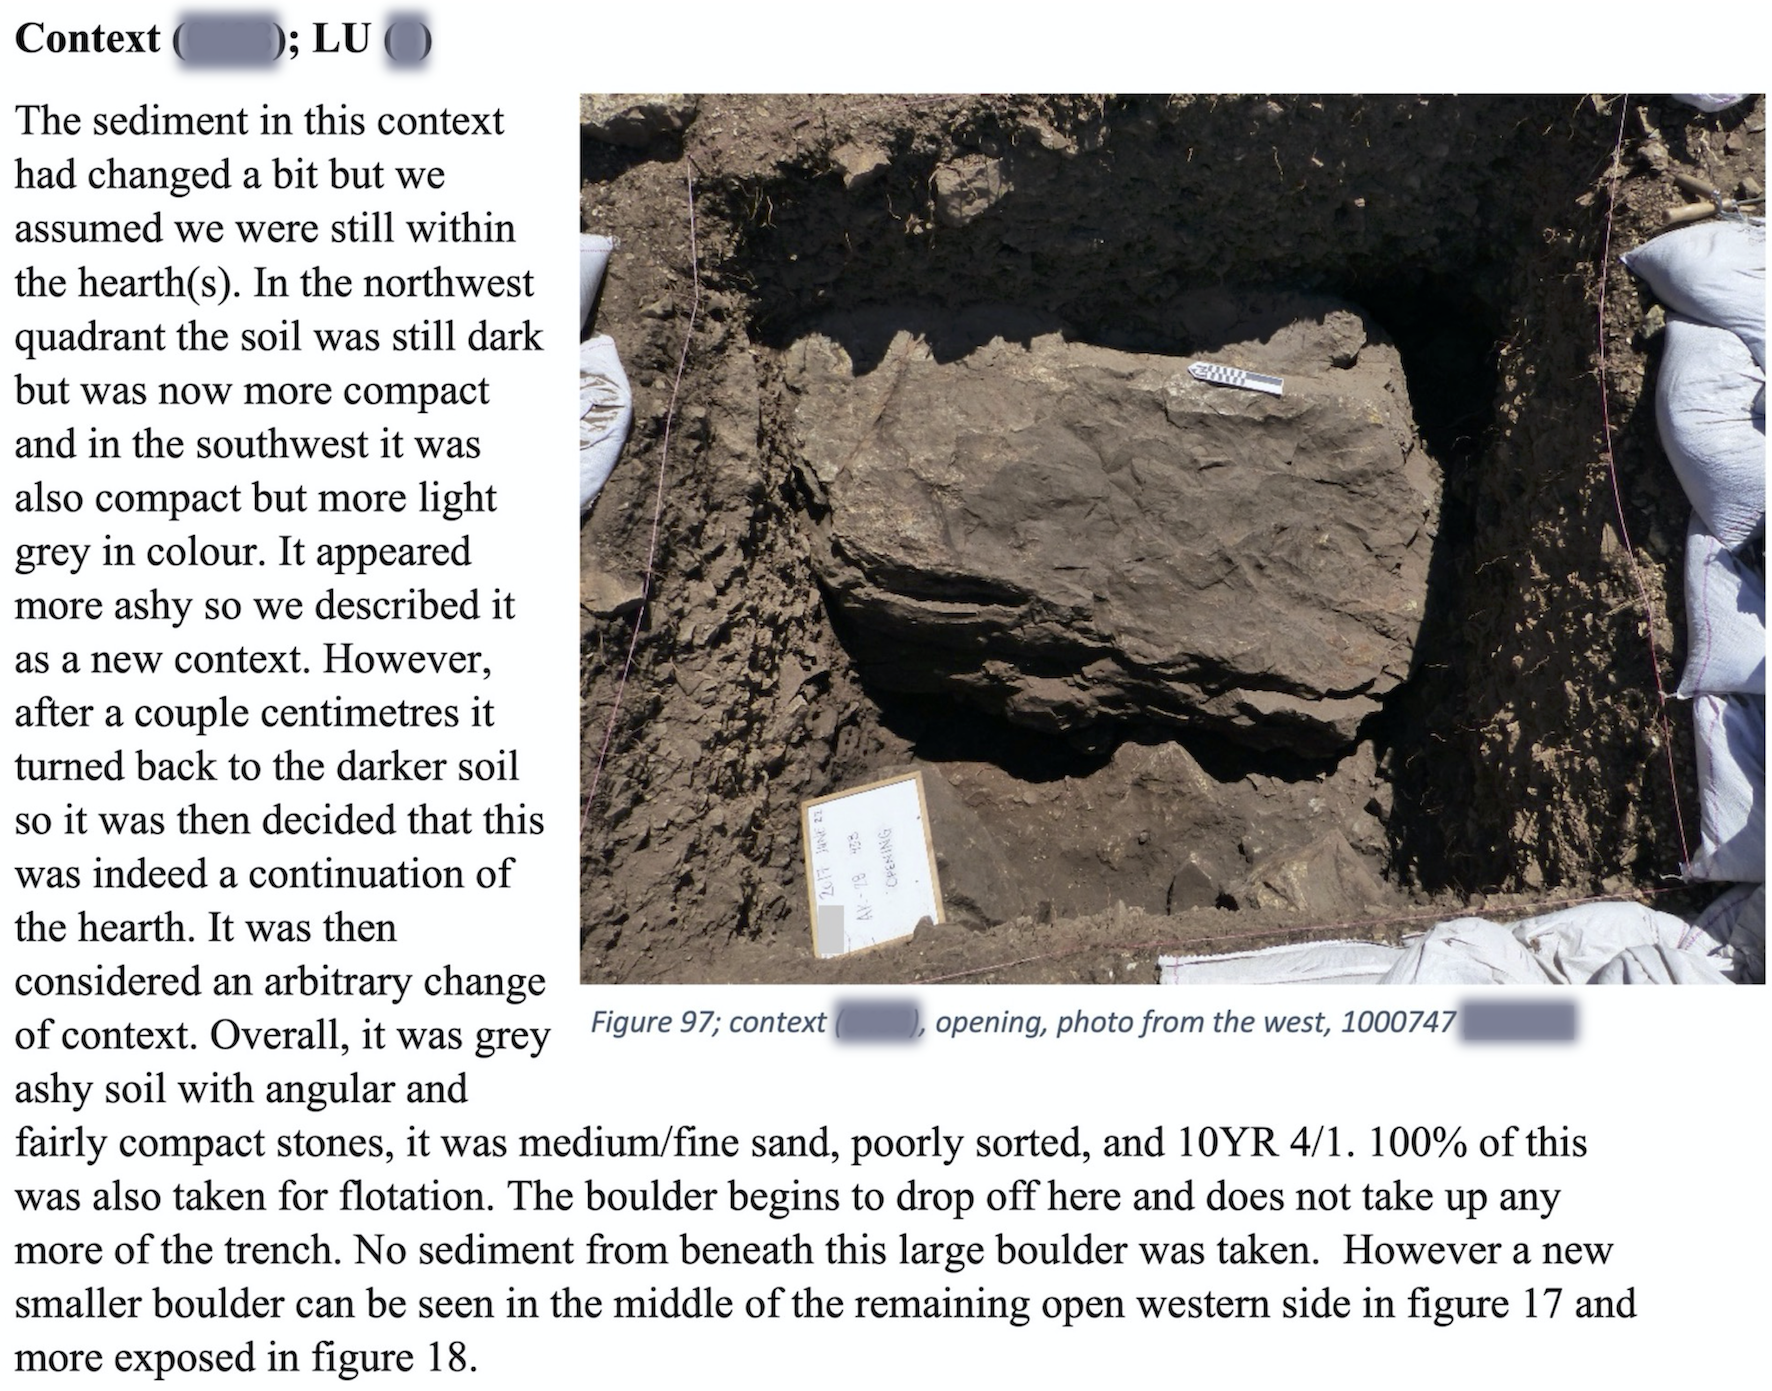
\includegraphics[width=0.99\textwidth]{context-report.png}
\caption{Section of a trench report describing the context addressed in the observed episode, and situating it as part of a lithostratigraphic unit.}
\label{fig:context-report}
\end{figure}

Moreover, the tentativity and ambiguity that Jane and Basil experienced while excavating this trench was one of its notable properties, as elicited in the final trench report (see \autoref{fig:context-report}).
Additionally, the report described how the contexts were eventually lumped together into a more concretely defined ``lithostratigraphic unit,'' which was formally delimited using nominal and standardized terminology.
In this way, the report switched back and forth between ambiguous and concrete representations, which conveyed experiential and distant perspectives, respectively.
This resembles the tone switching that occurred in the conversation between Jane and Basil, whereby Basil, as supervisor responsible for creating formal documentation, re-presented Jane's experiences using more formal terms.
As such, this reflects an implicit recognition that there is immense value in being able to share more nuanced perspectives on the things that make up the archaeological record (as per \cite[]{batist2024a}).

It is notable that situated experiences were recorded in the report-writing phase, and only by those acting in authoritative roles.
This parallels how field journals -- which are also records of situated experiences -- are exclusively maintained by supervising personnel \parencite[]{batist2024a}.
These observations reflect the different kinds of agency held by different actors in the project.
Fieldworkers were encouraged to shape their behaviour so that the information they obtained was born as formal entities from the start, whereas those responsible for presenting the record as part of a broader scope of work were responsible for re-situating the data as products of data-collection processes that they designed and dictated.
Recognizing the situatedness of data while they were being collected would have warranted recognition of their limitations, and was thought to enable undisciplined data collection behaviour.\textsuperscript{\ref{A20}}



